\subsection{Spectra}\label{sec:spectra}

Spectroscopy consists in the study of the radiative energy related to the wavelength.
An spectrum is normally obtained by observing a range of frequencies at the same time; 
it can be measured for example in radio wavelengths by a frequency sweep with 
a radio receiver or in visible and ultraviolet by the dispersion of the incident light 
through a diffraction grating or prism.
The analysis of the resultant spectrum can provide properties of the plasma observed 
such temperature, density, speed, etc.
Therefore, spectroscopy provides to the solar physicists invaluable information about 
the composition and the physical properties of the Sun.  

SunPy aims to provide support to most of solar spectroscopy instrument, however the 
complexity of this kind of datasets makes very challenging to add support to them all 
in a general way.  
Nevertheless, the \texttt{Spectra} object has been designed to be consistent with the 
other data types available in Sunpy.
It was implemented as a wrapper around a data array (numpy ndarray)
because its 1D nature (intensity versus frequency).
Using the \texttt{Spectra} object, Sunpy also offers a 2D array object called \texttt{Spectrogram},
which it is built as a group of spectrum meassured over time.
These two objects were implemented by funding provided by the Astrophysics Research 
Group at Trinity College Dublin.
As yet, Sunpy \texttt{Spectrogram} object supports radio spectra from the e-Callisto 
network\footnote{e-Callisto is an international network of solar radio spectrometers, 
                 all the data is available at: \url{http://www.e-callisto.org/} } 
and STEREO/SWAVES spectrograms.
Like for the \texttt{Lightcurve} object, the \texttt{Spectrogram} object has been
built so each instrument initialises from a sub-class containing the instrument-specific 
functionalities while offering common functionalities to them all to help its analysis, 
this includes:
read the data; %(fits format for e-Callisto, ASCII for STEREO/SWAVES); 
join different time ranges and frequencies; 
frequency dependent background subtraction;  
linearise of frequency axis and automated downsample for proper visualisation on a normal computer screen;  
and point-and-click functionality to save pixels of interest for further analysis.
In addition, this object is equipped with a download data interface for e-Callisto that 
only requires the observatory name and the desired time-range. 
STEREO/SWAVES data can be obtained via the virtual solar observatory (see \S\ref{ssec:vso}).

Listing \ref{code:spectra} shows how the \texttt{CallistoSpectrogram} object retrieves
from the online data archive the files that are between the time range specified and
the observatory of interest.  In this case the data is requested from \textit{BIR} which is the code name of the
Rosse Observatory at Birr Castle (Ireland)\footnote{\url{http://www.rosseobservatory.ie}}.
When the data is requested using the \texttt{.from\_range} function, the object merges
into a single spectrogram all the files downloaded, each with 15 minutes observation data 
and in some cases with different files for different frequency ranges.  
In the example shown here BIR observed in two frequency ranges: 20 - 90\,MHz and 55 - 355\,MHz.
Since the data is not evenly spaced in the frequency range, the \texttt{Spectrogram} object
linearise the frequency axis for a better analisys, as shown in the resultant figures.
It is also shown in the example the effect of the implemented background substraction and
\texttt{.peek} method.

\begin{listing}[H]
\begin{minted}[bgcolor=bg]{python}
from sunpy.spectra.sources.callisto import CallistoSpectrogram
tstart = "2011-06-07T06:00:00"
tend = "2011-06-07T07:45:00"
callisto = CallistoSpectrogram.from_range("BIR", tstart, tend)
callisto_nobg = callisto.substract_bg()
callisto.peek()
callisto_nobg.peek(vmin = 0)
\end{minted}
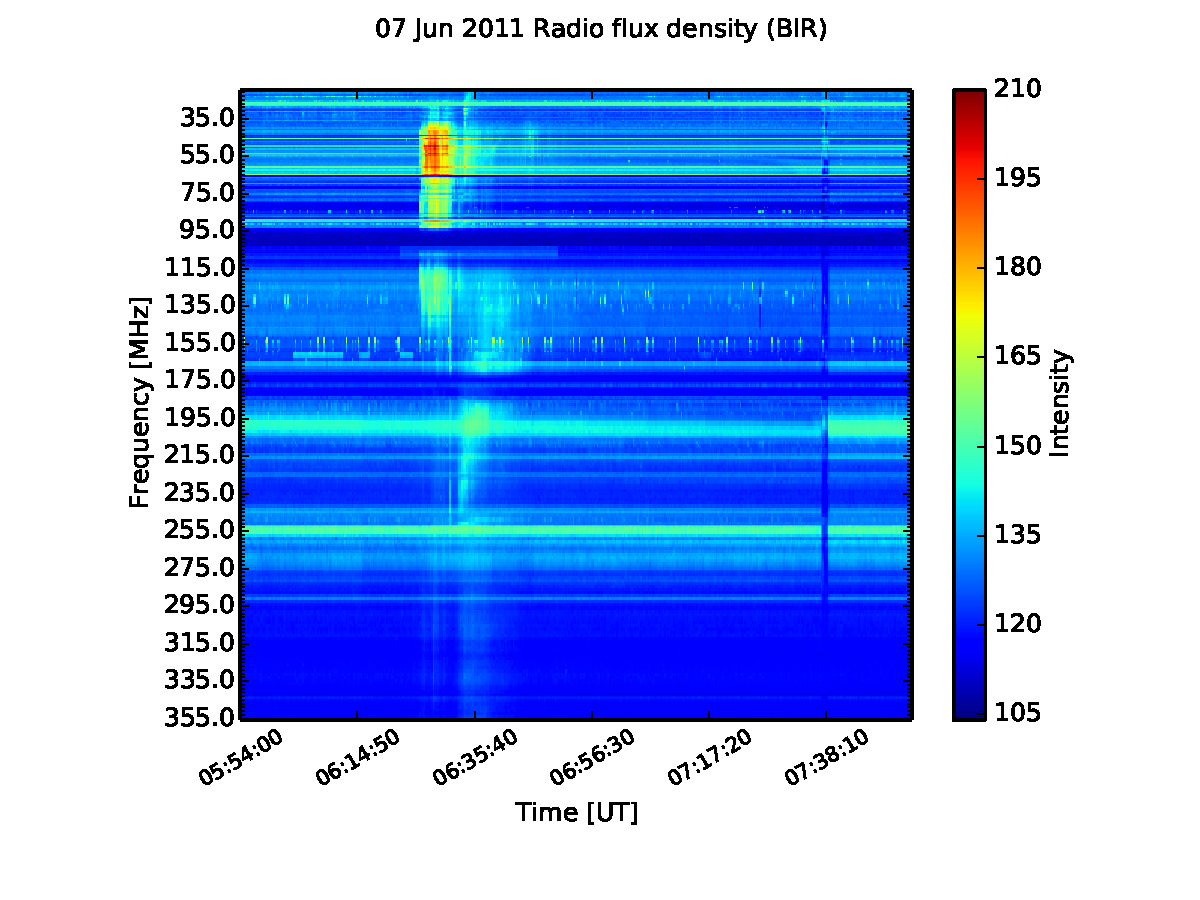
\includegraphics[width=0.8\columnwidth]{callisto} %\hfill
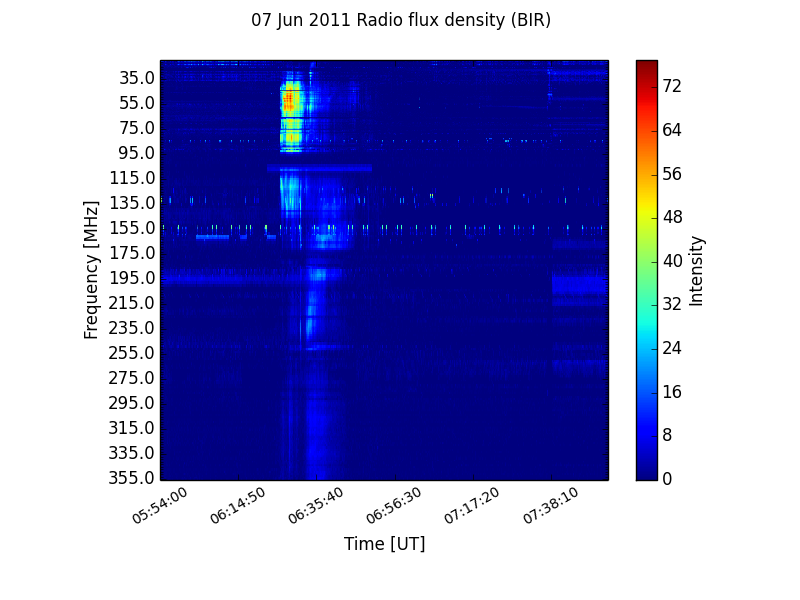
\includegraphics[width=0.8\columnwidth]{callisto_nobg}
\caption{Demonstration of how \texttt{CallistoSpectrogram} object retrieve the data
for the time range and observatory requested, merge it all and removes the background
signal.}
\label{code:spectra}
\end{listing}

% Download Callisto
% Merge multiple time-ranges / frequencies (just work from downlad!)
% Merge callisto with swaves

